%   *******************************************************************
%   * THIS IS THE MAIN FILE--RUNNING LATEX ON "AllegThesis.tex" WILL  *
%   * GENERATE THE ENTIRE THESIS (ASSUMING YOU HAVE NOT RENAMED IT).  *
%   * IF YOU ARE USING BIBTEX, RUNNING BIBTEX ON "AllegThesis" SHOULD *
%   * GENERATE YOUR BIBLIOGRAPHY. SPECIFIC DETAILS DEPEND ON WHAT     *
%   * ENVIRONMENT AND TOOLS YOU ARE USING (E.G., TEXMAKER OR COMMAND  *
%   * LINE TOOLS LIKE PDFLATEX OR ...).                               *
%   *******************************************************************
%
% AllegThesis.tex
% by A. Thall
% 13 Feb 2003
%
% Revised by R. Roos
% Nov 2013
%
% This document provides a sample Senior Thesis template for use
% by students in Allegheny's CS and Applied Computing programs.
%
%   *******************************************************************
%   * LOOK FOR BLOCK COMMENTS SUCH AS THIS ONE FOR AN EXPLANATION OF  *
%   * THIS DOCUMENT AND HOW TO MODIFY IT FOR YOUR OWN THESIS!         *
%   *                                                                 *
%   * ANY LINE BEGINNING WITH A "%" IS A LATEX COMMENT AND IS IGNORED *
%   * BY THE LATEX PROCESSOR. YOU ARE ENCOURAGED TO COMMENT YOUR OWN  *
%   * LATEX CODE TO HELP YOU REMEMBER WHY YOU DID THINGS A CERTAIN WAY*
%   *******************************************************************
%

%   ********************************************************************
%   * THE FIRST SECTION OF THE MAIN LATEX FILE IS THE "PREAMBLE." IT   *
%   * INSTRUCTS LATEX TO IMPORT SPECIAL PACKAGES FOR THINGS LIKE       *
%   * INCLUDING FIGURES, DOUBLE-SPACING, COLORED TEXT, ETC.            *
%   * DEPENDING ON YOUR NEEDS, YOU MAY FIND IT NECESSARY TO USE PACK-  *
%   * AGES THAT ARE NOT INCLUDED IN THIS TEMPLATE. SIMPLY IMITATE THE  *
%   * "\usepackage{...}" COMMANDS SHOWN BELOW.                         *
%   ********************************************************************

%   ********************************************************************
%   * BEGINNING OF PREAMBLE:                                           *
%   ********************************************************************

\NeedsTeXFormat{LaTeX2e}
\documentclass[12pt]{report}

%   ********************************************************************
%   * ALL BUT ONE OF THE FOLLOWING 5 LINES SHOULD BE COMMENTED OUT.    *
%   * (NOT ALL OF THESE OPTIONS HAVE BEEN TESTED IN THIS REVISION!)    *
%   ********************************************************************

%\usepackage[debug,draft,double]{gatorthesis} % for student proof doublespace
\usepackage[bottom,double]{gatorthesis} % for final department copy
%\usepackage[debug,draft,single]{gatorthesis} % for student workcopy
%\usepackage[single]{gatorthesis} % for student
%\usepackage[debug,draft,nolists,nofront,single]{gatorthesis} % more options


\usepackage{comment}     % provides a way to "comment out" sections in blocks
\usepackage{doublespace} % final document should be double-spaced!
\usepackage{amsmath}     % special symbols
\usepackage{amssymb}     % more special symbols
\usepackage{epsfig}      % needed for including figures
% \usepackage{fancybox}  % --- DISABLED BY RSR, SEP 2013 ---
\usepackage{url}
\usepackage{listings}
\usepackage[figure]{algorithm2e}
\usepackage{graphicx}

%   ********************************************************************
%   * OPTIONAL: IF YOU WANT VERY FINE CONTROL OVER HOW LATEX HYPHENATES*
%   * CERTAIN WORDS, YOU CAN PUT WORDS IN A "\hyphenation" COMMAND AS  *
%   * SHOWN IN THE FOLLOWING EXAMPLE. OTHERWISE, YOU MAY JUST IGNORE   *
%   * THE NEXT COMMAND.                                                *
%   ********************************************************************

% EXAMPLE: Don't hyphenate the words "itself" or "linear". Hyphenate 
%          "representations" only at the places indicated by the "-":

\hyphenation{itself repre-sen-tations linear state-ments career}

%   ********************************************************************
%   * THE FOLLOWING COMMAND HAS BEEN DISABLED--IGNORE.                 *
%   ********************************************************************
% The following provides a box to surround the thesis statement
%\newenvironment{Thesis}%
%{\begin{Sbox}\begin{minipage}{.95\linewidth}}%
%{\end{minipage}\end{Sbox}\begin{center}\fbox{\TheSbox}\end{center}}

%   ********************************************************************
%   ********************************************************************
%   ***  END OF PREAMBLE.                                            ***
%   ********************************************************************
%   ********************************************************************



%   ********************************************************************
%   * DOCUMENT CONTENT STARTS AT THE "\begin{document}" COMMAND:       *
%   ********************************************************************

\begin{document}

%   ********************************************************************
%   * FILL IN THE "{...}" BELOW WITH YOUR INFORMATION.                 *
%   ********************************************************************

\thesistitle{An Eclipse-based Integrated and\\Automated Fault Localization System}

\thesisauthor{Tristan Challener} \thesisadvisor{Dr. Gregory Kapfhammer}

\thesisnumber{CS15-02} 

\thesisreadera{Prof. John Wenskovitch}


%   ********************************************************************
%   * IN RARE CASES YOU MAY HAVE MORE THAN TWO READERS, IN WHICH CASE  *
%   * YOU SHOULD UN-COMMENT THE FOLLOWING AND ADD NAMES:               *
%   ********************************************************************
% \thesisreaderb{Dr. Your Thirdreader} 
% \thesisreaderc{Dr. Your Fourthreader}
% \thesisreaderd{Dr. Your Fifthreader}

%   ********************************************************************
%   * YOU MAY IGNORE THE FOLLOWING COMMAND:                            *
%   ********************************************************************
\date{\FileRevised \\ $\mbox{}$Revision: 1.8 $\mbox{}$}

\thesismaketitle         % Creates the title page
\thesismakecopyright     % Creates the copyright page

%   ********************************************************************
%   * YOU MAY SPLIT YOUR THESIS INTO SEVERAL FILES AND "\include" THEM *
%   * AS SHOWN BELOW. FOR INSTANCE, FILE "abstract.tex" CONTAINS THE   *
%   * ABSTRACT, FILE "ack.tex" CONTAINS THE ACKNOWLEDGMENTS, ETC. YOU  *
%   * MAY, OF COURSE, PUT EVERYTHING INTO ONE HUGE FILE, BUT THERE ARE *
%   * ADVANTAGES TO SPLITTING THINGS UP--FOR EXAMPLE, YOU CAN COMMENT  *
%   * OUT "\include" LINES OF SOME PARTS IN ORDER TO PRINT DRAFTS      *
%   * CONTAINING SELECTED SECTIONS OF YOUR THESIS, SAVING PAPER AND    *
%   * PRINTING COSTS.                                                  *
%   *                                                                  *
%   * YOU ARE NOT REQUIRED TO HAVE A "dedication"--IF YOU DON'T, JUST  *
%   * DELETE THAT LINE OR COMMENT IT OUT WITH A LEADING "%"            *
%   ********************************************************************

\begin{abstract}
Using \LaTeX\ to produce a professional-looking senior thesis can
be a daunting task. This work illustrates some of the more common
tools and features of \LaTeX. The PDF version of the thesis, together with
the heavily-commented {\tt .tex} source files used to produce it,
answer many questions commonly asked by
seniors concerning the final typeset thesis document.
\end{abstract}
  % REQUIRED!

% \include{dedication} % OPTIONAL

\chapter*{Acknowledgment}\label{ch:ack}
\addcontentsline{tob}{section}{Acknowledgment}

I like to acknowledge:

\begin{enumerate}

\item[]
Sarojini Balasubramanian, for providing the case application used in the study and the result files from running MAJOR on that application.

\item[]
Dr. Gregory Kapfhammer, for continuing advice and support, and for relentlessly forcing me to do my best.

\item[]
My colleagues, for advice, support, and patience throughout my Allegheny career.

\end{enumerate}
% \clearpage       % OPTIONAL, BUT ALMOST EVERYONE INCLUDES IT

%   ********************************************************************
%   * FRONT MATTER--TABLE OF CONTENTS, ETC. YOU PROBABLY DON'T NEED TO *
%   * CHANGE ANY OF THIS UNLESS YOU HAVE NO TABLES OR FIGURES, OR YOU  *
%   * WANT TO CHANGE NUMBERING DEPTH FOR SUBSECTIONS, OR ...           *
%   ********************************************************************

\setcounter{tocdepth}{2}    % # of section levels shown in table of contents
\setcounter{secnumdepth}{3} % # of numbered subsection levels in the text

\tableofcontents
\listoftables       % OMIT THIS IF YOU DON'T HAVE ANY TABLES
\listoffigures      % OMIT THIS IF YOU DON'T HAVE ANY FIGURES

%   ********************************************************************
%   * A GLOSSARY IS ALMOST NEVER NEEDED UNLESS YOU HAVE AN UNUSUALLY   *
%   * LARGE NUMBER OF SPECIAL TERMS OR NOTATIONS AND IT WOULD DETRACT  *
%   * TOO MUCH FROM THE FLOW OF THE PAPER TO DEFINE THEM IN-LINE.      *
%   ********************************************************************
%\include{glossary}  % OMIT THIS IF YOU DON'T HAVE A GLOSSARY (FEW PEOPLE DO)


%   ********************************************************************
%   * THE FOLLOWING "lstset" COMMAND IS ADAPTED FROM ONE FOUND AT:     *
%   * http://tex.stackexchange.com/questions/115467/                   *
%   * listings-highlight-java-annotations                              *
%   *                                                                  *
%   * SEE CHAPTER 3 AND APPENDIX A                                     *
%   ********************************************************************

\lstset{
  basicstyle=\footnotesize\tt, % the size of the fonts that are used for the code
  breakatwhitespace=false,     % automatic breaks only happen at whitespace?
  breaklines=true,             % sets automatic line breaking
  captionpos=b,                % sets the caption-position to bottom
  frame=single,                % adds a frame around the code
  language=Java,               % the language of the code
  keywordstyle=\bf,
  showspaces=false,
  showstringspaces=false,      % underline spaces within strings only?
  showtabs=false,
  tabsize=2                    % sets default tabsize to 2 spaces
}

%   ********************************************************************
%   * NOW INCLUDE THE CHAPTER FILES; COMMENT OUT ANY YOU DON'T WANT TO *
%   * PROCESS IN A PARTICULAR LATEX RUN.                               *
%   *                                                                  *
%   * INCLUDED FILES ARE ASSUMED TO END IN ".tex", E.G.,               *
%   * "ch01_overview.tex", "ch02_relatedwork.tex", ETC.                *
%   ********************************************************************

% ch:intro
%
% $Id: ch01_overview
%
%   *******************************************************************
%   * SEE THE MAIN FILE "AllegThesis.tex" FOR MORE INFORMATION.       *
%   *******************************************************************

\chapter{Introduction}\label{ch:intro} % we can refer to chapter by the label

The process of debugging can be complex and difficult.  The first task
associated with debugging is identifying the fault, and this step,
\emph{fault localization}, is the most expensive in terms of time cost
\cite{harrold}. In this chapter, we discuss current techniques for
fault localization and highlight the major goals of this
research project.

\section{Current State of the Art}\label{sec:state}
At present, the process of fault localization is mostly
manual, though several techniques exist that attempt to automate the
process.  A number of these techniques are described in detail below.
Many of these automated fault localization techniques (AFLs) compare the
flow of execution through a faulty program when executing passed and
failed test cases.  This type of approach employs \emph{coverage
monitoring}, the tracking of which statements are executed by test
cases.  Any statement that is executed is said to be \emph{covered}.
Tools such as Java Code Coverage (JaCoCo) \cite{jacoco} provide
information regarding which statements are covered by a supplied test
suite.  By analyzing code coverage for different test cases, these AFLs
seek to determine which statements are most likely to contain the fault.

Many coverage tools exist, including those designed for integrated development
environments such as Eclipse.  For example, JaCoCo provides interactive
coverage monitoring within Eclipse.  However, JaCoCo only reports total
coverage for a test suite; that is, the tool reports which statements
were covered, partially covered, or not covered after execution of all
of the test cases.  This system does not report on coverage of
individual test cases.  Since \emph{per-test coverage} is vital to the
application of several fault localization techniques, the lack of such
information leads to increased difficulty in applying those techniques.

As an alternative to the more popular JaCoCo, we will make use of a
lesser known tool called CodeCover.  Though a number of interfaces are
provided, including command-line and Apache Ant, we will focus on the
Eclipse plugin for the purpose of this project.  Unlike JaCoCo,
CodeCover is designed to produce coverage on a per-test basis.  The
system includes support for breaking coverage information for a JUnit 
test suite across test methods, automatically generating
distinct coverage data for each test method.  This functionality
makes CodeCover ideal to the goals of this project.

\section{Goals of the Project}\label{sec:goals}
There are two significant goals for this project.  The first is the
empirical evaluation of existing risk evaluation functions to 
determine the most effective on average.  This is a necessary step
in the process toward completion of our second goal, because no
study has made the specific comparison necessary.

The second goal of this project is the development of an Eclipse plugin
which displays the per-test coverage from a test suite and per-statement
suspiciousness analysis through an interactive system, as well as to
demonstrate its effectiveness.  The plugin will allow a programmer to
select individual or multiple test cases and view their coverage, or
to select individual statements and view a list of covering test cases
as well as suspiciousness rating and ranking. 

We hypothesize that making per-test coverage (in addition to suspiciousness
information), the basis for many fault
localization techniques, readily available will allow programmers to
more rapidly identify faults in programs.  This hypothesis will be
investigated through human study, employing experienced programmers
(specifically undergraduate students) to compare
the benefits of per-test coverage when compared to full suite coverage.
To generate test cases for evaluating our plugin, we will introduce
faults into programs using the MAJOR mutation analysis system
\cite{major}.

\section{Thesis Outline}\label{sec:outline}
This thesis consists of five chapters, which cover a wide variety of
topics related to the project.  In Chapter 2, we discuss past approaches
to problems in the area of fault localization.  In addition, we cover
existing tools which we will incorporate into our final system or make
use of to produce intermediate data.  Chapter 3 features a thorough
discussion of the method of approach used to achieve the results.  Specifically,
we relate the details of our test environment and setup for the empirical
comparison of risk evaluation functions, including test programs, method for
producing per-test coverage, and system for evaluating risk evaluation functions.
Chapter 3 also covers implementation details of the Eclipse plugin.

Chapter 4 provides the empirical results of the risk evaluation function
comparison study.  This includes various data visualization figures and
a discussion of these data.  We also discuss our conclusions as a result
of this study, as well as the impact these results have on our plugin 
implementation.  Chapter 5 discusses the human study used to evaluate our
plugin, beginning with the format and setup details and including the results
of the study.  We also discuss our conclusions based on the results of the study.
The final chapter reviews the project as a whole, annotates difficulties 
encountered, reiterates conclusions drawn in the previous chapters, 
and discusses future work. % Introduction -- of course, you can name it anything!

% ch:relatedwork
%
% $Id: ch02_relatedwork
%
%   *******************************************************************
%   * SEE THE MAIN FILE "AllegThesis.tex" FOR MORE INFORMATION.       *
%   *******************************************************************
\chapter{Related Work}\label{ch:relatedwork}

\section{Automated Fault Localization Techniques}\label{sec:afl}

There are a wide variety of existing fault localization techniques
\cite{harrold}. Many of these methods make use of per-test coverage
analysis, such as Set-union, Set-intersection, Nearest Neighbor, and
Tarantula.  There are other AFLs that do not use per-test coverage, such
as Cause Transitions \cite{cause}, but they are outside the scope of this project.  

Set-union and Set-intersection compare the coverage of a single failed
test case to the coverage of all of the passed test cases.  Set-union
defines the initial set of suspicious statements by the set of all test
cases visited by the failed test case but not visited by any passed test
cases.  Conversely, Set-intersection defines the initial set as the set
of all statements visited by every passed case but not by the failed
test case.  Nearest Neighbor works similarly to the previous techniques,
but instead of considering all of the passed test cases, it only
considers one.  By some method, the passed test cases that is most
similar to the failed test case is identified.  Nearest Neighbor defines
the initial set as the set of all statements visited by the failed case
and not by the passed case.

Tarantula is notably different from the previously mentioned techniques.
Instead of determining a set of suspicious statements, Tarantula ranks
techniques in order of suspiciousness.  However, Tarantula still
utilizes per-test coverage reporting.  In their paper, Jones and Harrold
present an empirical analysis which indicates the superiority of
Tarantula in both efficiency and effectiveness when compared to the
other techniques described above, as shown in Figure 1 \cite{harrold}.  Since Tarantula
uses per-test coverage, this provides substantial evidence for the
importance of per-test coverage in the fault localization process.

\begin{figure}
  \centering
  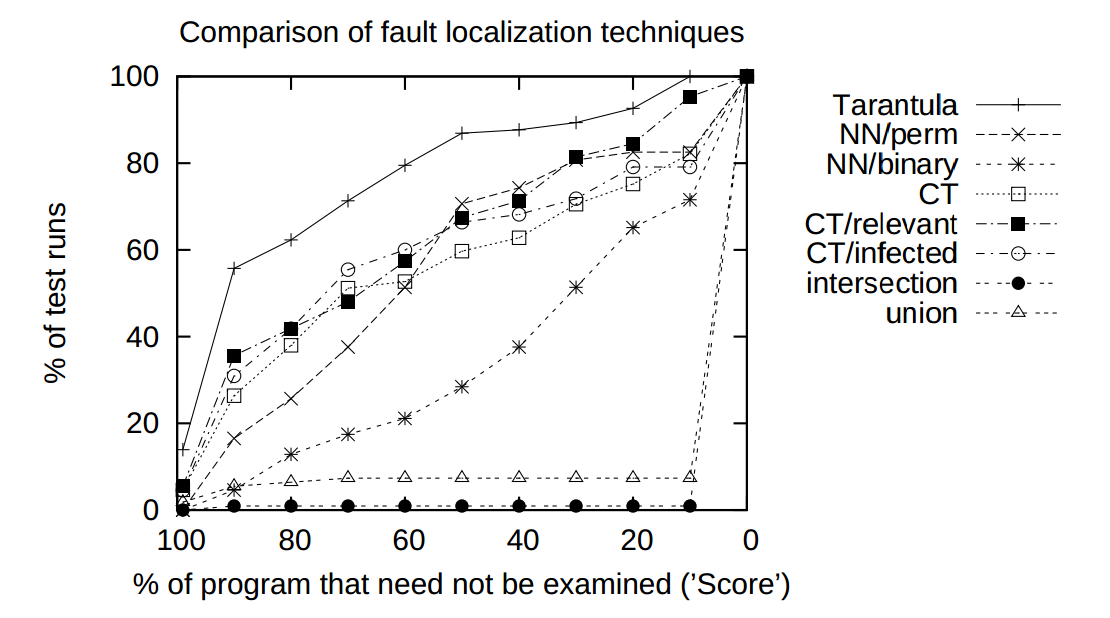
\includegraphics[width=0.9\linewidth]{img/tareff.png}
  \caption{An empirical comparison of several fault localization
  techniques by percentage of code eliminated from consideration.  The
  graph plots percentage eliminated (determined by the rank of the
  faulty statement) against frequency that the tool achieved that level
  of success.  Tarantula is demonstrated to achieve better results more
  often than other techniques.(from \cite{harrold})}
  \label{tareval}
\end{figure}

Xie et al. present an alternative discussion of various risk evaluation 
functions focusing primarily on theoretical correctness \cite{theory}. They 
argue that many existing risk evaluation formulas are actually functionally
equivalent.  In addition, they provide theoretical analysis that shows the 
superiority of specific functions relative to one another both within 
functionally equivalent groups and between those groups. Through detailed
theoretical proof they show that the equivalent sets ER1 and ER5 are maximal
for accurately calculating suspiciousness.  The ER1 set includes a pair of 
formulas studied in a paper by Naish et al. \cite{naish}  The ER5 equivalent 
set includes three functions, two of which are also studied in the paper
by Naish et al. The third is discussed in a paper by Wong et al. \cite{wong}
It is important to note that all the above risk evaluations also require
per-test coverage data.

As a followup to the paper by Xie et al. mentioned above, Qi et al. \hspace*{-0.7mm}\cite{genprog}
performed a detailed empirical to study the practical effectiveness of the 
theoretically maximal functions as proven by Xi et al.  This study includes
a wide variety of risk evaluation functions, and compares them by applying 
them to practical, real-world programs and faults.  The various formulas
were inserting them into popular automated program repair system GenProg.
GenProg uses genetic programming, applying a risk evaluation function to 
repeatedly alter a faulty program by mutating suspicious statements.  In their
study, Qi et al. \hspace*{-0.5mm}modified GenProg to use several different formulas.  By 
comparing the effectiveness of automated repair when using each different 
risk evaluation function, they were able to provide substantial empirical
evidence regarding the superiority of certain formulas.  Note that this method
of comparison differs from that pursued by Jones and Harrold \cite{harrold}, 
discussed previously, which compared the relative suspiciousness ranking of 
faulty statements (referred to as EXAM score).

Surprisingly, Qi et al. did not confirm the results shown by Xie et al.
Instead, they found that several functions, eliminated from consideration
as maximal functions early in the proof provided by Xie et al., were actually 
better than expected. Specifically,
Qi et al. show that in practice, the Jaccard risk evaluation function performed
equally as well or better than all other formulas considered.  They conclude that,
at least within the context of automated program repair, Jaccard should be 
favored when choosing a risk evaluation function.  In addition, they further 
conclude that the EXAM score method of comparing these formulas does not 
accurately reflect their relative performance in the context of automated
program repair.

In another paper \cite{parnin}, Parnin and Orso performed a human study about the
real-world effectiveness of fault localization techniques.  In that
study, they asked participants, graduate students in computer science
with varying levels of experience, to perform debugging tasks.
Participants were asked to compare their experiences when using standard
debugging practices with using an Eclipse plugin designed to display
Tarantula suspiciousness ranking.  This plugin was as simple as possible,
to eliminate from consideration any other factors besides suspiciousness
ranking.  The only functionality provided was a list of suspicious statements
which, when selected, navigated the environment to that line in the source
code.  When evaluating their hypotheses, he authors considered the
relative average amount of time required for each task, with and without
the plugin.  They also considered the relative experience level of the 
participants, which they evaluated based on number of tasks completed.  In 
addition, they also experimented with artificially raising and lowering
the rank of the fault statement in the suspicious statement list.  Finally,
Parnin and Orso used their plugin to record the order in which users
visited the suspicious statements, and asked the participants to complete
a questionnaire about their experiences and use of the tool.

Parnin and Orso came to a number of conclusions regarding several different
comparisons.  First, they noticed that in general, the participants did not
on average complete the tasks faster with statistical significance.  However,
they did notice a significant improvement in performance when using the tool
if the subject in question was more experience.  This suggests that, if the
tool were more refined and participants more used to the tool, it might actually
be significantly more helpful.  They also found evidence that suggests that the
exact rank of the statement does not significantly affect the difficulty of
locating the fault when using the tool.  In particular, participants often 
navigated the list of statements in a non-linear fashion: sometimes they skipped
ahead or backwards.  When skipping ahead, the authors suggest that participants
may have been skipping over code blocks they had already deemed unlikely to contain
the bug.  Finally, they conclude that there is no such thing as perfect bug 
understanding in practice.  That is, simply seeing a faulty statement out of 
context is not sufficient to identify and repair the bug.

We notice first that a large number of the negative results from Parnin and Orso's
study, in regards to the effectiveness of automatic fault localization, may have
stemmed from the simplicity of the Eclipse plugin tested.  We therefore hypothesize
that with a more sophisticated tool, programmers will have significantly improved
performance over use of traditional debugging techniques.  Since the goal of our
tool is to provide per-test coverage as context for suspiciousness, we suggest that
our tool is likely to outperform traditional debugging.

\section{CodeCover Coverage Analysis}\label{sec:cover}
CodeCover produces coverage information for Java, and has built in 
functionality for generating coverage information on a per-test suite,
per-test case, and even per-test method basis.  In addition, CodeCover
is designed to function within Eclipse.  All parts of the coverage
monitoring process can be done through the Eclipse development
environment.  Since the final goal of this project is to produce an
integrated Eclipse tool for fault localization, using per test
coverage and risk evaluation, CodeCover is ideally suited to our
purposes.  

\begin{figure}[htpb]
  \centering
  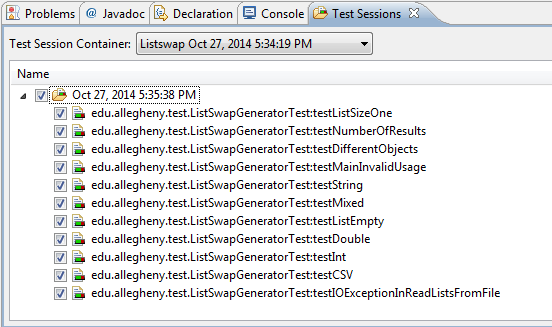
\includegraphics[width=4in]{img/codecoverpertest.png}
  \caption{Screenshot of CodeCover Eclipse plugin displaying per-test coverage
  output from a single execution of a JUnit test suite.}
  \label{codecover}
\end{figure}

CodeCover works in several stages.  The first step to acquiring coverage
information is instrumentation.  During instrumentation, numerous
statements are procedurally inserted into the Java source files which 
are to be included in the coverage analysis.  In the context of Eclipse,
these files are manually marked, since there may be source files for 
which coverage information is unnecessary.  The statements that are 
inserted during instrumentation record various information as the code
is executed, including which existing Java statements were executed, and
which test case or method exeucted them.  After instrumentation is
complete, the newly instrumented source files, as well as any other source
files, are compiled as normal.

CodeCover provides functionality for using existing JUnit test cases and
test suites for coverage analysis. With an existing Eclipse project with 
a JUnit test class, CodeCover can simply be enabled and executed.  By 
default, CodeCover produces output in the form of a several coverage
reports.  The output includes a full coverage report for every test method 
within the JUnit test; that is, per-test coverage data, as shown in Figure
\ref{codecover}.  

After executing a test process through the CodeCover Eclipse, per-test
coverage can be viewed in several ways.  First, coverage can be viewed on 
a per-test basis within Eclipse.  As shown in Figure \ref{codecoverage}, 
selecting one or more test methods displays coverage information for those
test methods only.  In addition to viewing coverage within Eclipse, CodeCover
allows coverage information to be executed in a variety of formats.  Using
provided template XML (eXtensible Markup Language) files, coverage data can be exported, for example, as
hierarchical HTML (HyperText Markup Language) documents or as CSV (Comma Separated Value) files.  

\begin{figure}[tpb]
  \centering
  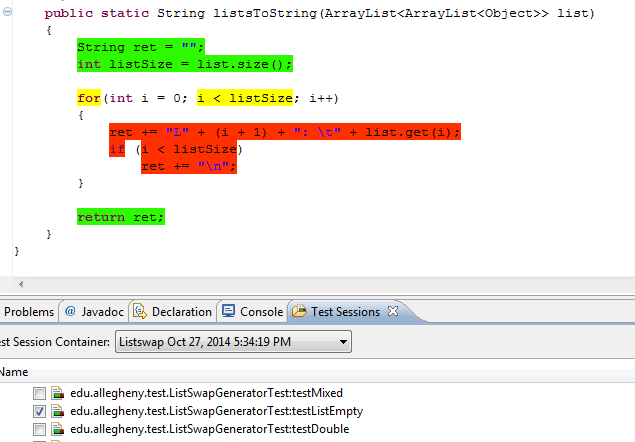
\includegraphics[width=4in]{img/codecovercoverage.png}
  \caption{Screenshot of CodeCover Eclipse plugin displaying coverage
  highlighting for a single test method.  Statements highlighted in green
  were covered by this test method, and those in red were not.}
  \label{codecoverage}
\end{figure}

\section{MAJOR Mutation}\label{sec:major}

MAJOR is a fault seeding and mutation analysis tool that integrates
directly into the Java compiler \cite{major}. \emph{Mutation} is the process of
intentionally introducing faults into a program for various purposes,
including evaluation of test suite quality and testing for fault
localization techniques.  Mutants generated are either \emph{killed} by
the test suite or \emph{live}.  A mutant is killed if a test case fails;
that is, the test suite was sufficient to identify the fault.  Live
mutants either indicate that the test suite is insufficient or that the
introduced fault was in fact logically equivalent to the original code.

MAJOR can perform a number of conditional mutations, including replacing
binary arithmetic, logical, relational, shift and unary operators with
valid alternatives.  Figure 4 shows an example of one
possible mutation performed by MAJOR.  The tool can also replace literal
values with alternatives; these various mutation types can be selected
with compiler operators.  Along with the domain specific language
provided by MAJOR, this allows for great flexibility and extensibility.
Additionally, MAJOR has been shown to be relatively efficient, with only
about 15\% runtime overhead.  It is also noteworthy that MAJOR utilizes
coverage analysis to improve efficiency.

A recent paper by Just et al. \cite{mutants} indicates a statistical
correlation between mutant detection and real world fault detection.
Although they also note that as much as 20\% of real world faults cannot
be represented by mutants, this still suggests that mutants are a viable
substitute for real world faults in the context of software testing and,
similarly, fault localization.

\begin{figure}[tbp]
  \centering
  \begin{lstlisting}
public static Type classify(int a, int b, int c) {
		int trian;
		if (a <= 0 || b <= 0 || c <= 0)
			return Type.INVALID;
		trian = 0;
	        ... (additional statements) ...
}
\end{lstlisting}

  \begin{lstlisting}
public static Type classify(int a, int b, int c) {
		int trian;
		if ((a <= 0 || b <= 0) != c <= 0)
			return Type.INVALID;
		trian = 0;
	        ... (additional statements) ...
}
\end{lstlisting}

  \caption{(top) Original program and (bottom) program after mutation.}
  \label{majorex}
\end{figure} % Background, literature survey, ...

% ch:method
%
% $Id: ch03_thework.tex
%
%   *******************************************************************
%   * SEE THE MAIN FILE "AllegThesis.tex" FOR MORE INFORMATION.       *
%   *******************************************************************
%
\chapter{Method of Approach} \label{ch:method}
In this chapter, we discuss the implementation details for our system.  The
implementation can be broken into four distinct sections:

\begin{enumerate}
\item XML parsing
\item Intermediate representation
\item Simplified representation
\item Risk evaluation
\end{enumerate}

\section{XML Parsing} \label{sec:parse}

When CodeCover produces per-test coverage information, it stores the results in
a container.  Though CodeCover features several coverage report export types, 
including hierarchical HTML, these reports do not include all information
necessary for this project.  Specifically, these export formals only include
general per-test coverage information, displaying percent coverage for each test.
They do not include information related to precisely which tests executed each 
statement, which is a requirement for suspiciousness analysis.  

Due to the limitations in CodeCover export formats, we are forced to make use of
the more complex XML container.  Since the container is in XML format, we must
first parse the file before we can perform analysis.  To that end, we utilize
DOM (document object model) parsing to store the entire container as a tree structure.  
We chose DOM over SAX(simple API for XML) due to the complexity of the container file.
Since SAX does not store the document in memory in its entirety, multi-pass analysis
is both more efficient and less complex when using DOM parsing.

\section{Intermediate Representation} \label{sec:ir}

After DOM parsing is complete, provided no errors occurred, the document tree root is
passed into the intermediate representation constructor.  The IR (intermediate representation)
for the container is designed to be simple to build while traversing a DOM of a CodeCover
container.  The \texttt{ContainerIR} object contains a list of \texttt{TestFile}s, as well
as a list of \texttt{String} names of test cases.  The object also includes a boolean values,
in which the $i^{th}$ element indicates the pass/fail status of the $i^{th}$ test case.  A 
visualization of the container IR, as well as its internal data structures, can be found in 
Figures \ref{fig:ir} and \ref{fig:ir2} respectively.  

\begin{figure}[tb]
\centering
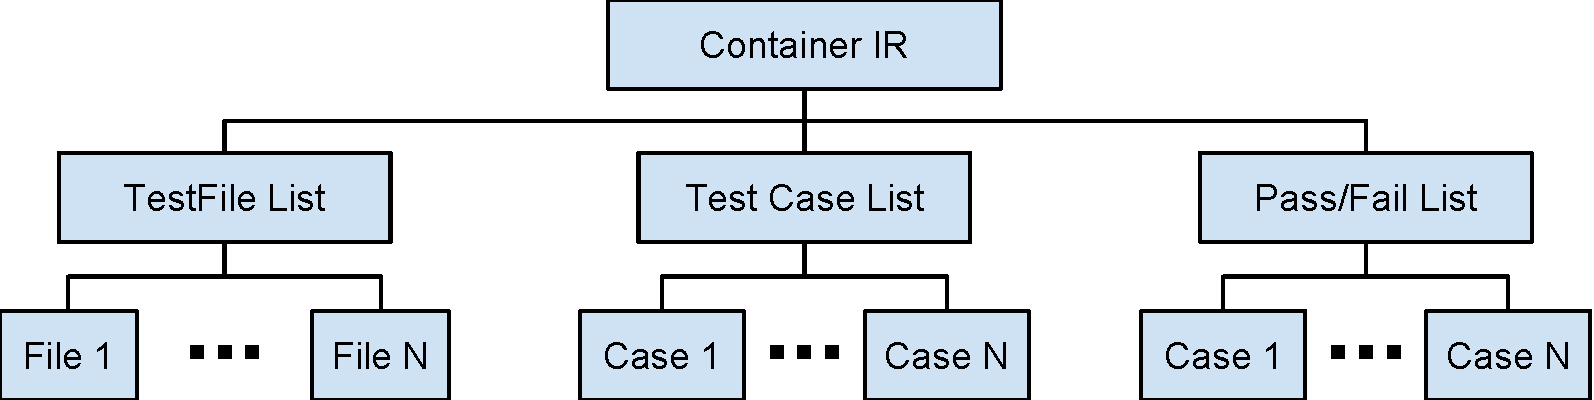
\includegraphics[width=0.8\linewidth]{img/ContainerIR.pdf}
\caption{Diagram of data structure for IR.}
\label{fig:ir}
\end{figure}

\begin{figure}[tb]
\centering
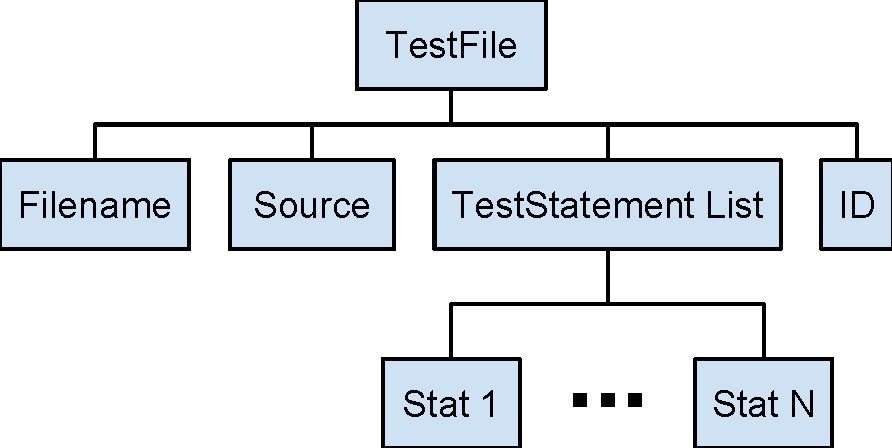
\includegraphics[height=30mm]{img/TestFile.pdf}
\hspace{0.1\linewidth}
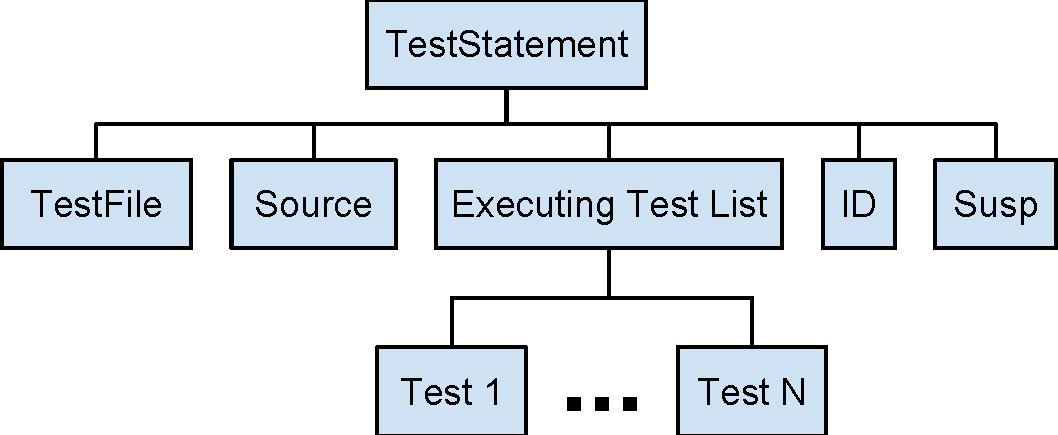
\includegraphics[height=30mm]{img/TestStatement.pdf}
\caption{Diagram of data structures used within the IR to store files (left) and 
statements (right)}
\label{fig:ir2}
\end{figure}

Each \texttt{TestFile} object contains the name and source code of the file as a \texttt{String}, the internal identification numberfor the file as an \texttt{int}, and a list of \texttt{TestStatement}s.  
A \texttt{TestStatement} includes an ID and source code for the statement, each stored as \texttt{String}s.  In addition, the \texttt{TestStatement} object stores a \texttt{TestFile} 
parent object and the suspiciousness value associated with the statement.  Finally, the statement 
includes a \texttt{boolean} list, where each element corresponds to a test case.  These boolean 
values indicate whether the respective test case executed this statment.  A \texttt{TestStatement} 
can be uniquely identified by the combination of its source file and ID.

CodeCover coverage containers include all required
information, divided into three sections.  First, the container lists all source
files included in coverage analysis, including the entirety of their source code,
the name of the file, and a unique internal identification value.  Following the source files
is a hierarchical list of all statements within those files.  These statements are defined by 
by their category, source file, and character offset within the source file.  For this
project, we only consider basic statements (in Java, this essentially refers to executable
statements terminated with semicolons).  

The final section of a CodeCover container is the per-test coverage data itself.  This is
represented by a series of test cases, each of which contains a child for every file
executed by that test. Under each file is a list of specific statements executed by that
test inside that file.  These statements are identified by their alphanumeric identifier.

Our system processes these sections in the order they appear above.  Using the DOM produced
from parsing, we can easily traverse the relevant segments of the container.  Traversal of
the DOM tree consists of repeated iterations of sub-levels of the XML hierarchy, in order
to locate a node with a specific name.  Throughout this process, we make no assumptions about
the sequence in which nodes appear.  Rather than assume that, for example, a given node is
always the first child, we always use a loop structure to make certain we identify the correct
node.

In order to identify all source files defined by the
XML container, we first locate the \texttt{SrcFileList} node.  We then iterate through its
children to locate all \texttt{SrcFile} nodes.  For each \texttt{SrcFile} node found, we 
extract the attributes of that node and add a \texttt{TestFile} to the \texttt{ContainerIR}
file list.  

Once we have located the source files, we must next identify the statements.  To do so, we first
locate the hierarchical statement definition root.  Beginning with that root node, we recursively
traverse the entire sub-tree.  For each \texttt{BasicStmnt} node, we add a new statement to the 
correct \texttt{TestFile}.  In order to do so, we must first identify the \texttt{LocList} child
node, followed by its \texttt{Loc} child node.  The attributes of the \texttt{Loc} node include
the source code character offset for the basic statement in question.  Between the attributes of
the \texttt{BasicStmnt} node and those of the \texttt{Loc} node, we extract the information
necessary to create a new \texttt{TestStatement} object.  Once this recursive traversal of the
statement hierarchy is complete, the \texttt{TestFile}s in the \texttt{ContainerIR} will contain
all basic statements.

Since we now have a complete list of basic statements, we can process the coverage data section
of the container to identify test cases and their coverage.  To begin, we first iteratively 
locate the \texttt{TestSession} node, whose children include a \texttt{TestCase} node for
each test case in the test suite.  We add the name of each test case to the \texttt{ContainerIR}
test case list, then process the children of the node to find coverage data.  Each test case
node contains a hierarchy of \texttt{CovList}, \texttt{CovPrefix}, and \texttt{Cov} nodes.  We 
locate all \texttt{CovPrefix} nodes, which each correspond to a single file, then retrieve the
\texttt{TestFile} corresponding to this node from the list of test files within the \texttt{ContainerIR}.
Finally, we iterate through all \texttt{Cov} children of the \texttt{CovPrefix} to find all 
basic statements covered by a given test case within a given file.  For each statement identified,
we mark the corresponding \texttt{TestStatement} as covered.

In addition to coverage data, a \texttt{TestCase} node also contains a \texttt{Comment} attribute.
This content of this attribute is comprised of the entire text output produced when the test case
was executed.  When the test case passes, this attribute is empty; however, when a failure occurs,
the description of the failure is stored in this node.  As a result, we can observe this attribute
to determine the pass/fail status of a given test.  We ascertain this data by checking the
\texttt{Comment} attribute for the starting string \texttt{"Failure"}.  Since this word always
heads the description of a failure, the \texttt{Comment} of a failed test will always begin with
the same text.  This pass/fail value is recorded in the boolean list stored in the 
\texttt{ContainerIR}, where true indicates a passed test and false indicates a one in which a failure
occurred.

\section{Simplified Representation} \label{sec:sir}

The intermediate representation discussed in section \ref{sec:ir} is appropriate as a preliminary
data structure.  However, it is not conducive to suspiciousness analysis.  All of the risk evaluation
functions considered in this project require four pieces of information for each statement that
must be evaluated: $ae_f, ae_p, an_f, \text{ and } an_p$ \cite{theory}.  These variables represent the number
of test cases that meet certain requirements for a given statement.  Variables $ae_f$ and $ae_p$
denote the number of test cases that executed the given statement and failed or passed
respectively. Similarly, $an_f$ and $an_p$ refer to the number of test cases that did not execute
the statement and passed or failed, respectively.  These four values become the input to each of
the suspiciousness functions.  Therefore, the simplified representation that best suits our needs
is one that stores these values for each statement, with no extraneous information.

In order to convert the IR to the described simple representation, the first step is build
a list of \texttt{TestInfo} objects, which represent individual test cases.  Each \texttt{TestInfo}
object includes a pass/fail boolean value, as well as a boolean list that describes, for each
statement under test, whether that statement was executed by this test.  We extract this information 
from the IR by iterating through the list of test case names.  For each test case, we check the
execution status of that test case for each statement, storing this information in a list (where
each element corresponds to a single statement, and true indicates the statement was executed by this
test).  Next, we cross check that test case index with the corresponding element in the pass/fail
boolean list in the IR and set the pass/fail status of the new \texttt{TestInfo} object to reflect
that value.

Iterating through the \texttt{TestInfo} list, we can determine the $ae_f, ae_p, an_f, \text{ and } an_p$
of each statement.  For each test case, we check whether the test passed then determine which statements
it executed by iterating through the boolean list stored in the \texttt{TestInfo} object.  For each
statement, we increment the appropriate variable depending on its pass/fail and execution status.  The
result is a list, for each of the four variables, in which each element corresponds to its value for
the corresponding statement.  After completing this process, we have a \texttt{CoverageReport} object
with all of the information necessary for risk evaluation.

\section{Risk Evaluation} \label{sec:re}

There are many different risk evaluation functions, but they are structurally similar.  We internally
represent risk evaluation functions using our \texttt{REFunction} interface.  This interface provides
abstract methods for returning the name of the function and for evaluating the function on provided
$ae_f, ae_p, an_f, \text{ and } an_p$.  Figure \ref{fig:re} provides an example implementation of
the REFunction interface.  For each function included, we create an implementation of
\texttt{REFunction}.  A complete list of \texttt{REFunctions} is stored in a static array of the
same name in \texttt{CoverageReport} for ease of iteratively performing all evaluation functions.  

\begin{figure}[tb]
\centering
\begin{lstlisting}
public class Jaccard implements REFunction {
	public double analyze( int aef, int aep, int anf, int anp ) {
		return ( (double) aef / (aef + anf + aep ) );
	}

	public String toString() {
		return "Jaccard";
	}
}
\end{lstlisting}

\caption{Implementation of REFunction interface for Jaccard function.}
\label{fig:re}
\end{figure}

When performing risk evaluation, we iterate through the specified functions.  For each of these
functions, we store the results of analysis in a \texttt{ResultsList} data structure.  This
structure allows for ease of sorting analyzed statements by suspiciousness rating.  In addition, the
suspiciousness values of the \texttt{ResultsList} are normalized to a zero-to-one scale according to

\[ L_i = \frac{ L_i - L_{min} }{ L_{max} - L_{min} }. \]

In this equation, $L_i$ refers to the $i^{th}$ element of the \texttt{ResultsList}, and $L_{max}, L_{min}$ refer to the maximum and minimum values in the list, respectively.  Though normalizing the results does
not change the ordering of the statements, it does make the actual suspiciousness values easier to compare
across multiple different functions.  The final result of analysis is a list of statements, ordered from
most suspicious to least suspicious, with values ranging from zero (not suspicious) to one (very 
suspicious).

\section{Overview} \label{sec:over}

When executing the system, the main class, \texttt{Test.java}, must be invoked with three additional
parameters.  The first of these is the fully qualified name of the JUnit test class (e.g. \texttt{edu.allegheny.listswap.ListSwapGeneratorTest}), which will be programmatically executed to
obtain pass/fail information.  This test class \emph{must} be in the classpath, or the system will
not be able to execute the tests.  The second parameter is the fully qualified file name for the 
CodeCover container to be analyzed.  The final parameter is the name for the output file---the 
output path is fixed to the (to be created) results directory within the present working directory.

Execution begins with parsing the XML container.  When the document has been stored as a DOM, it is
passed forward to the \texttt{ContainerIR} constructor, which processes the document into an IR as
described previously.  The IR is then passed to the \texttt{CoverageReport} class, where the 
test class is executed and coverage information is collated into the simple representation.
Suspiciousness evaluation is then completed using all risk evaluation functions specified.

After performing suspiciousness evaluation, the results are written to an output file in CSV (comma
separated value) format.  The attributes \textit{Function, Statement ID, Filename, Suspiciousness, Rank,
Statement Count,}
and \textit{Case Application} serve to uniquely identify a statement while providing information on risk evaluation.  
This format conforms to \textit{tidy data}  \cite{tidy}, a ``standard way of mapping the meaning of a 
dataset to its structure'', in that each variable forms a column and each observation forms a row.  
This organizational structure allows for reliably simple evaluation of data using statistical 
analysis tools.  Though tidy data contains extensive redundancy, that redundancy simplifies
the data analysis and visualization process.

%\section{Test Environment}
%Algorithm \ref{widgmin} (from \cite{Fiori:2013}) shows a high-level description of an
%algorithm. There are many options for the display of
%pseudocode; this uses the {\tt algorithm2e} package \cite{Fiori:2013}, 
%but there are a number of others available at the Comprehensive \TeX\ Archive
%Network (\url{ctan.org}). Using any of these
%other packages might require the additon of one or more
%``\verb$\usepackage{...}$'' commands in the main {\tt AllegThesis.tex} file.
%
%%   *******************************************************************
%%   * SEE CHAPTER ch_01overview.tex FOR INFORMATION ON CONTROLLING    *
%%   * PLACEMENT OF FIGURES.                                           *
%%   *                                                                 *
%%   * THERE ARE MANY DIFFERENT ALGORITHM ENVIRONMENTS. HERE, WE USE   *
%%   * THE "algorithm2e" PACKAGE, BUT YOU SHOULD LOOK TO SEE IF        *
%%   * OTHER PACKAGES BETTER MEET YOUR NEEDS. REGARDLESS OF WHICH      *
%%   * PACKAGE YOU USE, EXPECT TO SPEND TIME READING THE USER MANUAL   *
%%   * AS THERE ARE USUALLY A LARGE NUMBER OF PARAMETERS THAT CAN      *
%%   * SIGNIFICANTLY AFFECT THE FINAL APPEARANCE OF THE ALGORITHM.     *
%%   *******************************************************************
%
%\begin{algorithm}[htbp]
% %\SetLine % For v3.9
% \SetAlgoLined % For previous releases [?]
% \KwData{this text}
% \KwResult{how to write algorithm with \LaTeX2e }
% initialization\;
% \While{not at end of this document}{
%  read current\;
%  \eIf{understand}{
%   go to next section\;
%   current section becomes this one\;
%   }{
%   go back to the beginning of current section\;
%  }
% }
% \caption{How to write algorithms (from \cite{Fiori:2013})}
%\label{widgmin}
%\end{algorithm}
%
%\section{Experiments}
%
%Figure \ref{javaprog} shows a Java program. There are many, many options for
%providing program listings; only a few of the basic ones are shown
%in the figure. Some thought must be given to making code suitable
%for display in a paper. In particular long lines, tabbed indents, and
%several other practices should be avoided. Figure \ref{javaprog} makes
%use of the {\tt listings} style file \cite{Heinz:2013}.
%
%%   *******************************************************************
%%   * SEE CHAPTER ch_01overview.tex FOR INFORMATION ON CONTROLLING    *
%%   * PLACEMENT OF FIGURES.                                           *
%%   *                                                                 *
%%   * SEE THE MAIN FILE "AllegThesis.tex" FOR THE "\lstset" COMMAND   *
%%   * THAT DEFINES HOW PROGRAM LISTINGS WILL LOOK.                    *
%%   *                                                                 *
%%   * AS WITH EVERYTHING IN LATEX, LOOK AT THE USER MANUAL, SEARCH    *
%%   * FOR EXAMPLES ONLINE, CUSTOMIZE TO GET A PLEASING LOOK.          *
%%   *******************************************************************
%
%
%\begin{figure}[htbp]
%\centering
%\lstinputlisting{SampleProgUncommented.java}
%\caption{{\tt SampleProg}: A very simple program}
%\label{javaprog}
%\end{figure}
%
%\section{Threats to Validity}
%
 % Chapter organization is topic-dependent

%ch:implem
%
% $Id: ch04_implementation.tex
%
%   *******************************************************************
%   * SEE THE MAIN FILE "AllegThesis.tex" FOR MORE INFORMATION.       *
%   *******************************************************************
%
\chapter{Experimental Results}\label{ch:results}

In this chapter, we will discuss our method of verifying the accuracy of our system,
a discussion of our case study, an analysis of the results produced by our system,
and a listing of possible threats to the validity of our results.

\section{Testing}\label{sec:test}

Throughout the development process, we used several mechanisms to verify the accuracy
of our system.  Prior to starting implementation, we selected a very simple sample
program to ensure that we could use CodeCover to produce per-test coverage data.  The
program we selected was a small system developed by Nathaniel Blake, Tristan Challener, 
and Eric Weyant as a course project at Allegheny College.  The system consists of four
source files and eleven JUnit test cases, and has functionality related to file input,
list manipulation, and CSV output.  We selected this application primarily for its
simplicity, existing JUnit test suite, and our familiarity with the code.  Its
simplicity allowed us to easily import the system to Eclipse and set up the environment
to successfully run all included tests.  This process was aided by our familiarity with
the code and tests; although we did not have to modify any executable code or the 
content of any tests, we were required to update certain aspects of the tests to behave
correctly on a Windows operating system.

After importing our selected application into Eclipse, we installed the most recent version
of the CodeCover Eclipse plugin.  By following directions provided in the CodeCover documentation,
we were able to execute the application through CodeCover and produce per-test coverage data.
Because CodeCover containers are internal mechanisms for storing coverage data and are not
meant to be viewed directly, there is very little documentation available.  As such, we were 
forced to examine the container output to determine its structure before developing parsing
tools.  See Section \ref{sec:ir} for additional details about the content of CodeCover
container files.

As we proceeded with the implementation described in Chapter \ref{ch:method}, we cross-checked
the data produced from our parse tool with that available through interacting with the CodeCover
Eclipse plugin.  We were able to verify that our parsed coverage data was consistent
with the data shown in Eclipse.  Verifiable data included statement source code, execution 
counts for each statement, and test case pass/fail status.  In addition, we verified the values
generated for $ae_p, ae_f, an_p,$ and $an_f$ through manually totaling the number of appearances 
of each statement in the container coverage segment to the values of each of the aforementioned
variables.  

Through these processes we were able to establish a reasonable level of confidence
in the correctness of our system.  Automated testing was not a feasible option for this process
due to the complex nature of the container being parsed, since any testing would require 
repeating the parsing process---thereby negating the benefits of the test.  Automated testing
was used, however, to verify the accuracy of the risk evaluation function implementations
used in the system.  We designed table-driven JUnit tests with multiple test inputs to 
ensure that all functions were correctly implemented within a reasonable degree of confidence.

\section{Case Study}\label{sec:case}

In order to provide further evidence for the accuracy of our system and to produce preliminary 
comparison data for our tested risk evaluation functions, we performed a case study with another
selected application. Due to the simplicity of the test application described in Section \ref{sec:test}, 
we chose a different case application for our study.  The program we selected is Jni-InChi
\cite{jniinchi}, which ``enables Java software to generate IUPAC's International Chemical Identifiers 
(InChIs) by making Java Native Interface (JNI) calls to the InChI C library developed by IUPAC''.

This application, along with several others, was prepared and executed through MAJOR by Sarojini
Balasubramanian.  The mutation data were provided as well.  We selected this application, from the
several other applications available, due to limitations of CodeCover that were not clear until we
began testing various applications.  Many tested applications had passing JUnit test suites after
being imported to Eclipse, but still produced the following (or similar) error when we attempted
to run them through CodeCover:

\vspace{5mm}
\texttt{[FATAL] An error occurred when trying to compile the instrumented sources.}
\vspace{2mm}

According to a discussion post at the CodeCover \texttt{sourceforge}
page, made by CodeCover developer Tilmann Scheller \cite{discpost}, there is not currently any 
means of producing more verbose output (including details on compiler errors) through Eclipse.  
Additional discussion indicated that CodeCover is able to ``instrument
a single source directory only.''  Since the majority of the projects provided and executed with MAJOR
feature several source directories, we were severely limited in choice of case study application.  
Fortunately, the Jni-InChi project includes only a single source directory and we were able
to generate CodeCover output for this system.

\begin{figure}
\centering
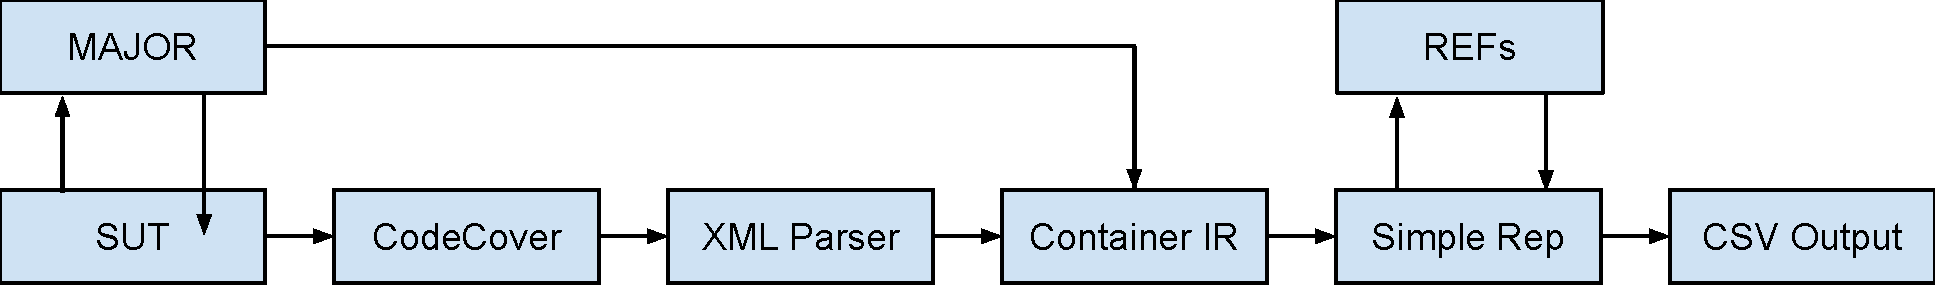
\includegraphics[width=0.9\linewidth]{img/Architecture.pdf}
\caption{The overall architecture of the system for experimentation.  The system under test (SUT) is executed through MAJOR, and some fault is inserted.  The SUT then passed through CodeCover, and the resulting container forms the input to the XML parser.  The parsed container, and the fault, are passed into the IR builder.  Once the IR is built, it is passed to the simplified representation (SR) modifier.  The SR calls all of the necessary risk evaluation functions (REFs), then outputs the results to CSV.}
\label{fig:arch}
\end{figure}

In order to produce meaningful results, the CodeCover execution of JUnit must complete or no coverage
data is written to the container.  Additionally, the JUnit test must
feature at least one failure---otherwise no
suspiciousness information can be generated.  To achieve this, we repeatedly selected
arbitrary \textit{killed} mutants generated by MAJOR (their killed status guarantees at least one failed
test case).  As mentioned earlier, mutants have been shown to be representative of real-world faults.  
Specifically, mutants generated using MAJOR were shown to be representative in the study by Just et al.
\cite{mutants}  The overall layout of this test is visualized in Figure \ref{fig:arch}.

\begin{figure}[tb]
\begin{lstlisting}
119:ROR:==(java.lang.Object,java.lang.Object):
	FALSE(java.lang.Object,java.lang.Object):
	net.sf.jniinchi.JniInchiAtom@<init>:117:el == null |==> false
137:STD:<CALL>:<NO-OP>:
	net.sf.jniinchi.JniInchiStructure@addBond:99:
	bondList.add(bond) |==> <NO-OP>
149:LVR:POS:NEG:
	net.sf.jniinchi.JniInchiStereo0D@<init>:79:3 |==> -3
194:COR:||(boolean,boolean):LHS(boolean,boolean):
	net.sf.jniinchi.JniInchiWrapper@checkOptions:183:
	op.startsWith("-") || op.startsWith("/") |==> op.startsWith("-")
197:STD:<CALL>:<NO-OP>:
	net.sf.jniinchi.JniInchiWrapper@checkOptions:189:
	sbOptions.append(flagChar + option.name()) |==> <NO-OP>
\end{lstlisting}

\caption{Mutants selected for use in case study.}
\label{fig:mutants}
\end{figure}

There were various complications that forced us to reject mutants.  First, any mutant that
causes the Eclipse JUnit \texttt{TestRunner} to crash prematurely and not complete the entire test 
suite could not be used.  This is due to meaningless or incomplete coverage data, which is not useful
for generating suspiciousness data.  In many cases, if the \texttt{TestRunner} crashed prematurely,
CodeCover would not write \emph{any} coverage data to the test session container.  Thus, we skipped
any mutants with this property. We also passed over any mutants that modify non-executed code, such
as static variable declarations.  
This makes mutants of this type invalid for the purpose of suspiciousness analysis.  Any remaining
mutants were considered valid.  From those not disqualified, we chose five arbitrary mutants to 
form the basis for this case study.   These mutants can be seen in Figure \ref{fig:mutants}.

Since we only consider basic statements when parsing the CodeCover container, inserted mutants
must be formatted in such a way that they occur as a Java statement and get parsed by CodeCover
as basic statements.  For \texttt{<NO-OP>} mutants such mutant 137, we achieved this by replacing
the listed line with a statement that does nothing.  Specifically, we insert a local variable 
initialization an always-false \texttt{if} statement making use of that variable (if the variable
is never referenced, CodeCover will not recognize the initialization as a basic statement).  That 
variable initialization is treated as the faulty treatment, effectively simulating a no-operation
statement.  Mutants which modify the condition inside an \texttt{if} statement can be represented by 
moving the condition to a boolean variable declared and initialized directly before the \texttt{if}
statement.  That boolean variable initialization is treated as the faulty statement.  The remaining
mutant, number 149 as labeled in Figure \ref{fig:mutants}, requires no additional modifications since
it directly alters a basic statement.

When CodeCover processes source code and builds a test session container, it copies the entire source
code into the container, but removes all comments from the content.  As such, line numbers and character
offsets within CodeCover are not comparable to those within the original source code.  In
order to locate the inserted fault within the container, we require the source code for the faulty
statement to be included as an input to our system, as described in Section \ref{sec:over}.

\section{Results Analysis}\label{sec:data}

In order to process the data produced by our system for the case application, we made use of the
R functional language for statistical computing \cite{r}.  Since our data already conforms
to tidy data standards \cite{tidy}, and is formatted as CSV, it was relatively simple to import the
data directly into R.  We begin our analysis by reading each CSV results file into a single 
\texttt{data.frame}.  We then vertically merge all of the resulting tables into a single table with
the same variables, but including all observations rather than only those for a single case 
application (mutation).  After merging the tables, we add the EXAM score for each statement to the table 
as a new variable, calculated according to \[EXAM = \frac{Rank}{StatementCount} \times 100.\]

Before making any further use of the data, we create a new table consisting only of the statements
which correspond to the fault.  This is accomplished by selecting only observations from the table
in which the \texttt{IsFault} attribute is true.  We then break this table down into five smaller tables according to the risk evaluation function.  For each of the resulting tables, we extract the 
\texttt{Exam} attribute vector and calculate its mean (the average EXAM value for a given function
across all case applications).  Using these average values, we construct a new table consisting only
of the attributes \texttt{Function} and \texttt{Exam}, made up of five observations---one for each
function and its corresponding average EXAM value.  The final step before visualization is to 
recreate the original five tables, with EXAM values added, by splitting the large table according to
case application.

\begin{figure}[tb]
\centering
\begin{lstlisting}
library( ggplot2 )
attach( jniinchi_119_fault )
graph_119 <- qplot( Function, Exam, data=jniinchi_119_fault, geom="bar", 
			  	ylab="EXAM Score (%)", xlab="Risk Evaulation Function", 
				stat="identity", ylim=c( 0,5 ),
				main="EXAM Score Per Risk Evaluation Function (JniInChi Mutant 119)",
				sub="JniInChi Mutant 119" )
graph_119 <- graph_119 + theme( axis.title=element_text( face="bold.italic" ) )
detach( jniinchi_119_fault )
\end{lstlisting}

\caption{Example code for generating visualization of results.}
\label{fig:rgraph}
\end{figure}

For each of the five case application tables, as well as the average EXAM value table, we produce a
single bar graph.  To do so, we utilize the \texttt{qplot} function from the \texttt{ggplot2} library
\cite{ggplot2}.  The bar graphs plot EXAM score against risk evaluation function, each displaying the
performance of every risk evaluation function for a different case application.  The final graph plots
the average performance of each function across all mutations.  The code used to generate one of the
graphs can be seen in Figure \ref{fig:rgraph}.

\begin{figure}[tb]
\centering
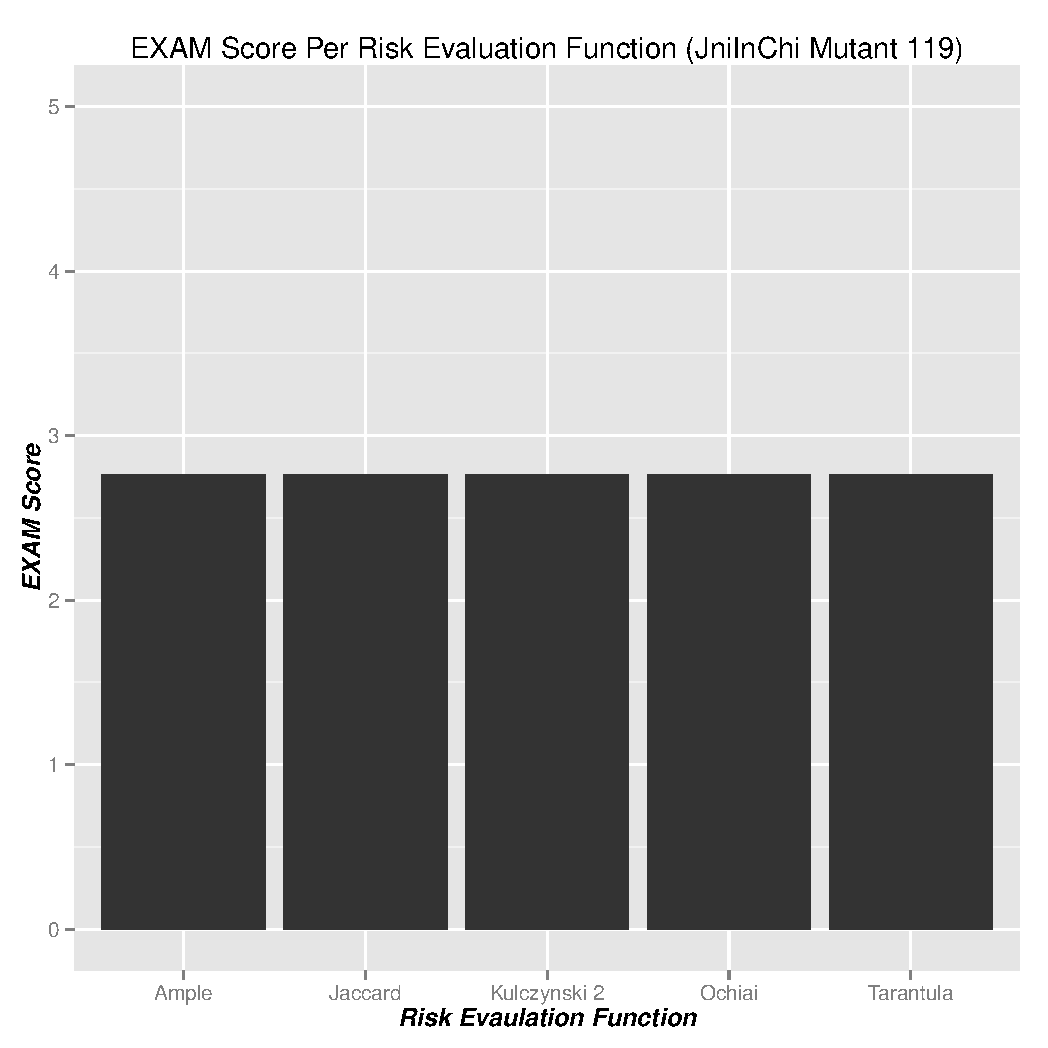
\includegraphics[width=0.4\linewidth]{img/graph_119.pdf}
\hspace{0.1\linewidth}
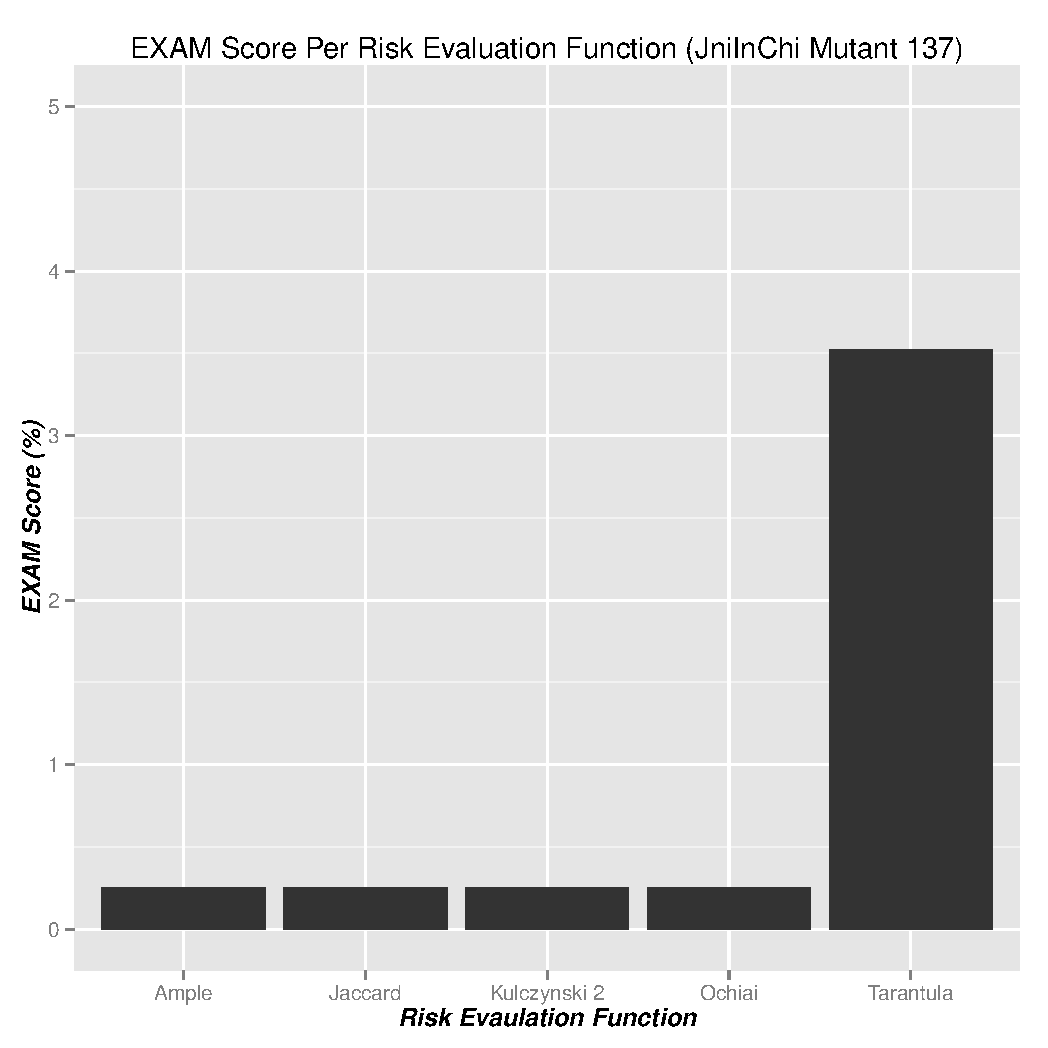
\includegraphics[width=0.4\linewidth]{img/graph_137.pdf}

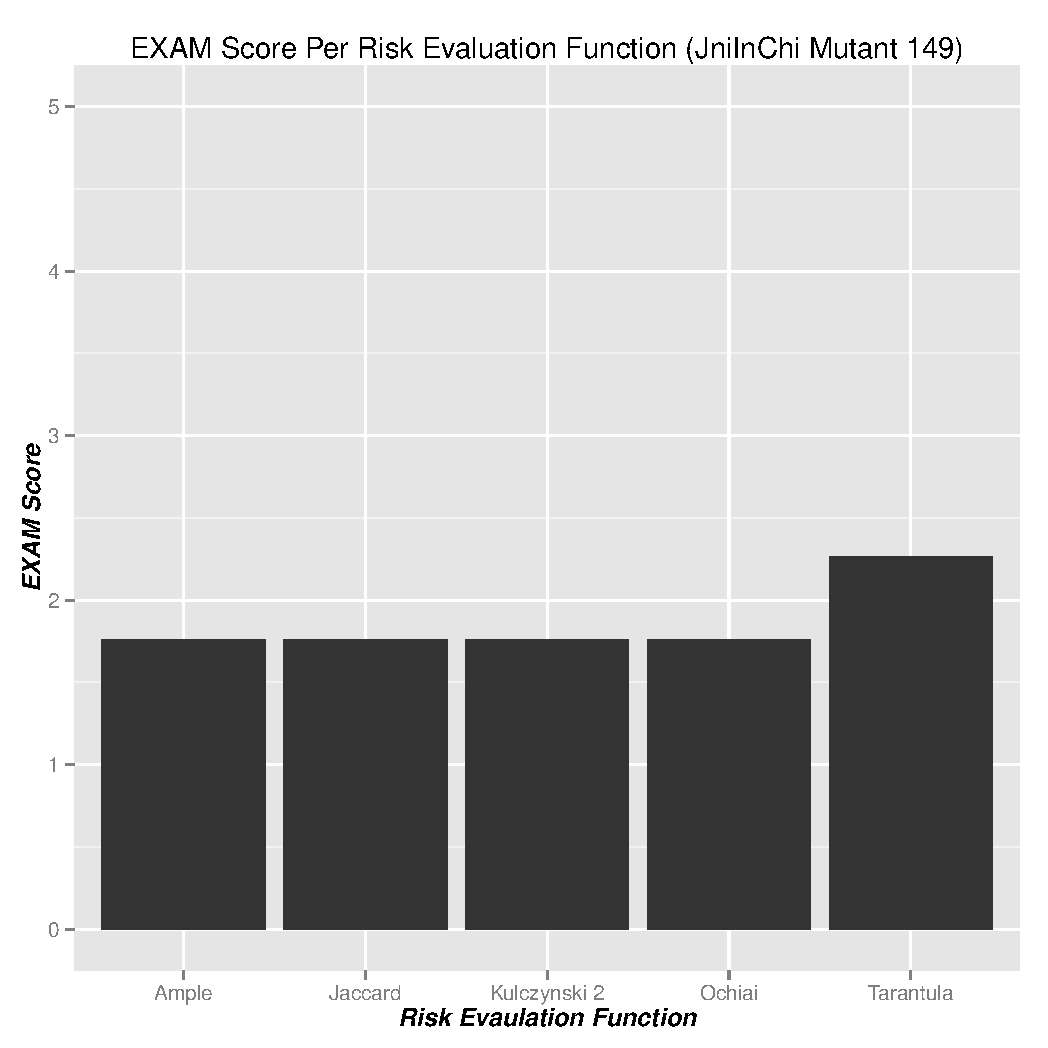
\includegraphics[width=0.4\linewidth]{img/graph_149.pdf}
\hspace{0.1\linewidth}
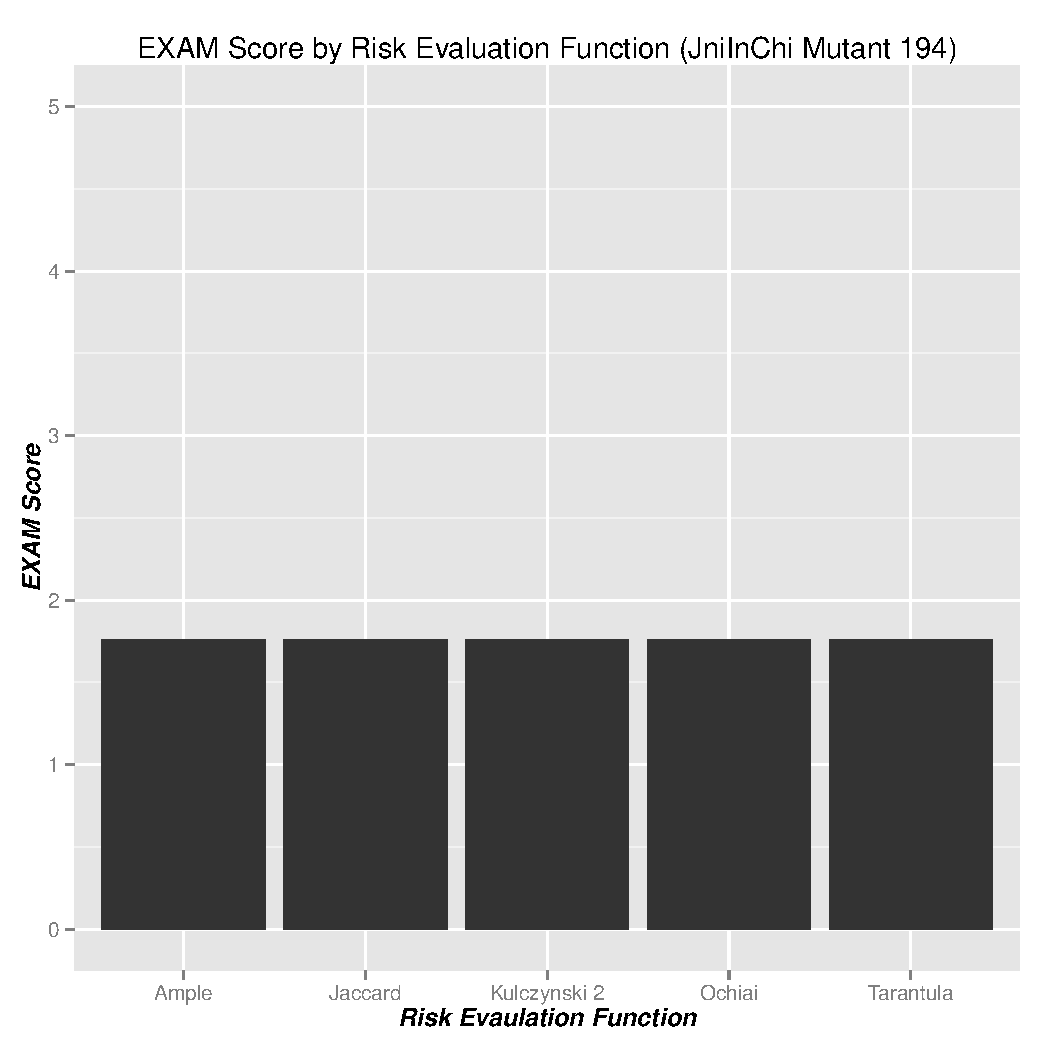
\includegraphics[width=0.4\linewidth]{img/graph_194.pdf}

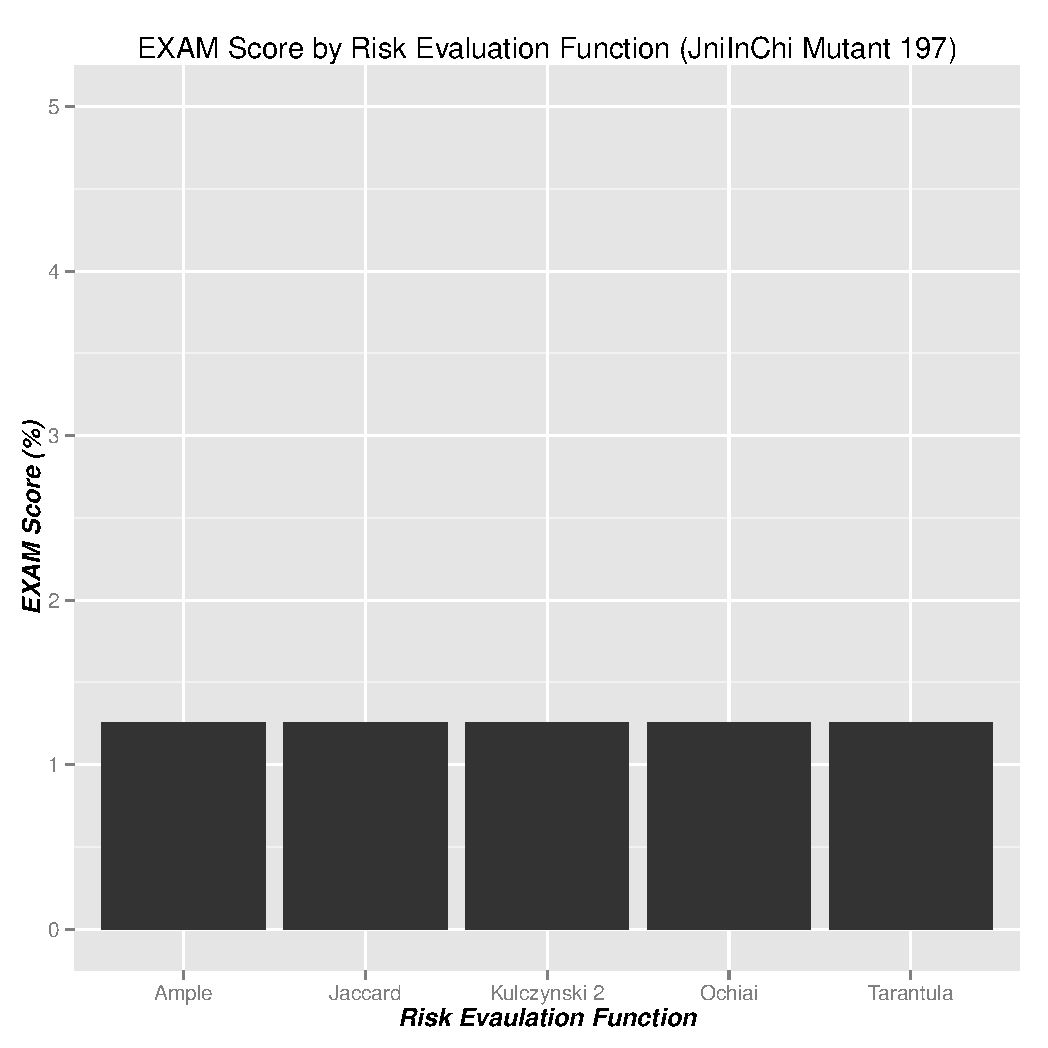
\includegraphics[width=0.4\linewidth]{img/graph_197.pdf}
\hspace{0.1\linewidth}
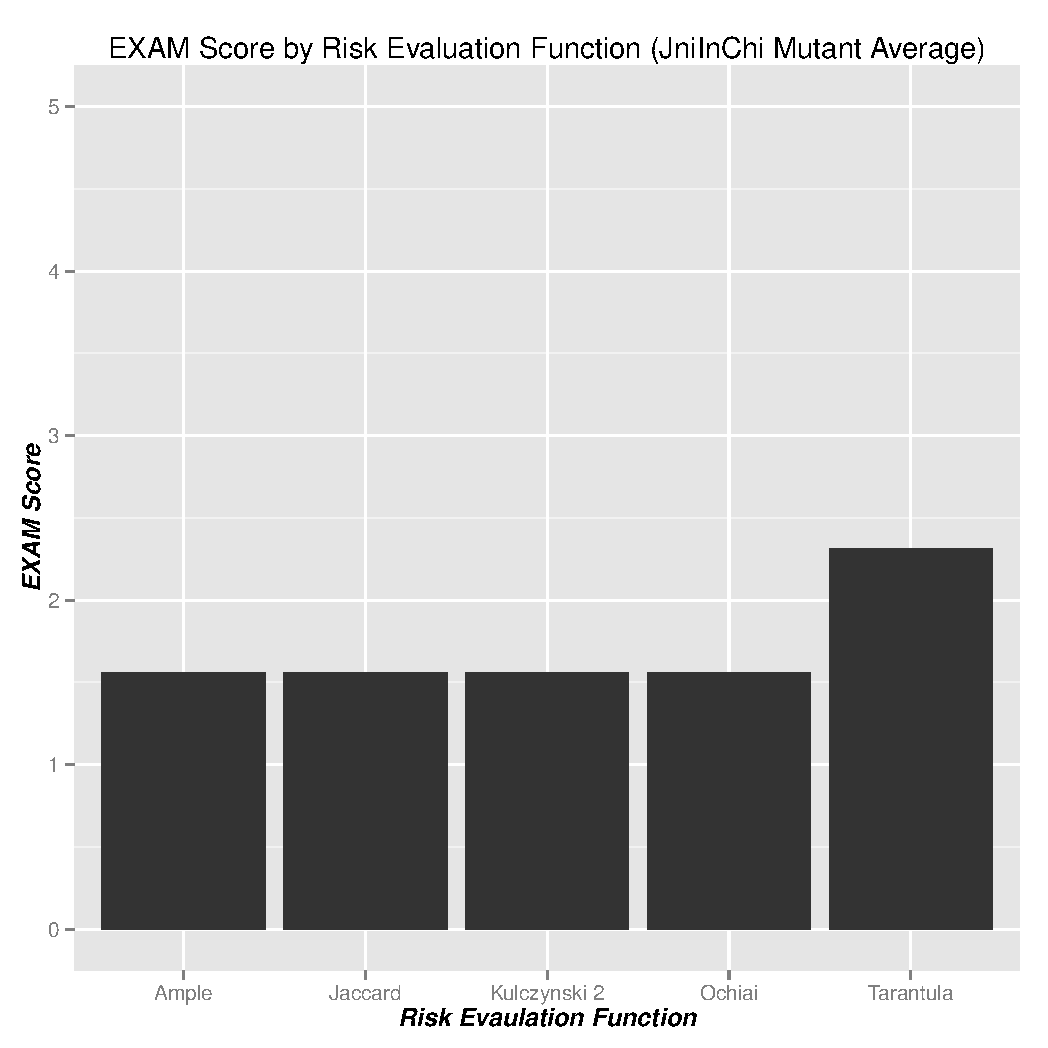
\includegraphics[width=0.4\linewidth]{img/graph_avg.pdf}

\caption{Graphs produced through R showing the results of running
the system on each selected mutation on our case study.  Each graph
shows the EXAM score achieved by each risk evaluation function for a
different mutant, with the exception of the last (lower right) which
shows average EXAM score overall for the case application.  All graphs
are fixed to the same EXAM range from 0\% to 5\%.}
\label{fig:results}
\end{figure}

The bar graph visualization of our results is can be found in Figure \ref{fig:results}.  For nearly every case, 
we notice that every risk evaluation function performed nearly or exactly the same.  Though the 
graph for Jni-InChi mutant 137 appears to be wildly skewed, it is important to note that the range of the
graph only covers five percent.  Even in the worst case, none of the risk evaluation functions scored
worse than 3.5\%.  Recall from Section \ref{sec:afl} that EXAM score is a lower-is-better metric
indicating the percent of statements that need to be visited, when proceeding sequentially through a 
list of suspicious statements, before encountering the actual faulty statement.


\section{Threats to Validity}\label{sec:valid}

Due to complications related to the use of CodeCover to generate per-test coverage, we were only able
to produce results for a single case application.  As such, we can only provide a certain degree of
confidence in the correctness and versatility of our system for processing CodeCover containers.  However,
after testing and developing the system with a very simple application, no modifications were necessary
to process the far more extensive output generated when running CodeCover on our case application.  This 
allows us to conclude that we can be reasonably confident that our system will likely work for any
coverage container.  The difficultly, then, lies in the limited capacity of CodeCover to produce 
output for a wide variety of source applications.

 % Chapter organization is topic-dependent

%ch:conclusion
%
% $Id: conclusion.tex
%
%   *******************************************************************
%   * SEE THE MAIN FILE "AllegThesis.tex" FOR MORE INFORMATION.       *
%   *******************************************************************
%

\chapter{Discussion and Future Work}\label{ch:conclusion}

In this chapter we discuss the significance of our results and review
important underlying assumptions that may affect the relevance of results.
In addition, we discuss future work that may follow directly from the 
results and conclusion to this project.  Finally, we summarize the
important points presented throughout this thesis.

\section{Summary of Results}

\section{Future Work}

\section{Conclusion}
 % Conclusion/future work

%   ********************************************************************
%   * IF YOU HAVE ANY APPENDICES (FOR INSTANCE, CODE, DATA, GRAPHS,    *
%   * OR ANYTHING ELSE THAT DOESN'T "FIT" AS REGULAR CHAPTER CONTENT), *
%   * INCLUDE THE FOLLOWING LINE, WHICH INSTRUCTS LATEX TO CHANGE FROM *
%   * NUMBERED "CHAPTER" HEADINGS TO LETTERED "APPENDIX" HEADINGS.     *
%   *                                                                  *
%   * APPENDICES HAVE THE SAME FORMATTING COMMANDS AS CHAPTERS (E.G.,  *
%   * "\chapter{...}", "\section{...}", ETC.)                          *
%   ********************************************************************

\appendix

%
% $Id: appa--code
%
%   *******************************************************************
%   * SEE THE MAIN FILE "AllegThesis.tex" FOR MORE INFORMATION.       *
%   *******************************************************************

\chapter{Java Code}\label{appa:code}
All program code should be fully commented. Authorship
of all parts of the code should be clearly specified. 

%   *******************************************************************
%   * SEE THE MAIN FILE "AllegThesis.tex" FOR THE "\lstset" COMMAND   *
%   * THAT DEFINES HOW PROGRAM LISTINGS WILL LOOK.                    *
%   *******************************************************************

\lstinputlisting{SampleProg.java}

  % Source code

%
% $Id: appa--code
%
%   *******************************************************************
%   * SEE THE MAIN FILE "AllegThesis.tex" FOR MORE INFORMATION.       *
%   *******************************************************************

\chapter{Source Code}\label{appb:code}

%   *******************************************************************
%   * SEE THE MAIN FILE "AllegThesis.tex" FOR THE "\lstset" COMMAND   *
%   * THAT DEFINES HOW PROGRAM LISTINGS WILL LOOK.                    *
%   *******************************************************************

This appendix contains all source code for our system.  Source code is
included in alphabetic order by class name.  The source can also be found in
its entirety within our GitHub repository, which is located at:\\ \url{https://github.com/challenert/cs600f2014-challenert}

\section{System Code}\label{sec:cov}

\lstinputlisting{C:/Users/Tristan/workspace/Comp/src/edu/allegheny/cov/Ample.java}
\lstinputlisting{C:/Users/Tristan/workspace/Comp/src/edu/allegheny/cov/ContainerIR.java}
\lstinputlisting{C:/Users/Tristan/workspace/Comp/src/edu/allegheny/cov/CoverageReport.java}
\lstinputlisting{C:/Users/Tristan/workspace/Comp/src/edu/allegheny/cov/Jaccard.java}
\lstinputlisting{C:/Users/Tristan/workspace/Comp/src/edu/allegheny/cov/Kulczynski2.java}
\lstinputlisting{C:/Users/Tristan/workspace/Comp/src/edu/allegheny/cov/Ochiai.java}
\lstinputlisting{C:/Users/Tristan/workspace/Comp/src/edu/allegheny/cov/ParseContainer.java}
\lstinputlisting{C:/Users/Tristan/workspace/Comp/src/edu/allegheny/cov/REFunction.java}
\lstinputlisting{C:/Users/Tristan/workspace/Comp/src/edu/allegheny/cov/ResultsList.java}
\lstinputlisting{C:/Users/Tristan/workspace/Comp/src/edu/allegheny/cov/Tarantula.java}
\lstinputlisting{C:/Users/Tristan/workspace/Comp/src/edu/allegheny/cov/Test.java}
\lstinputlisting{C:/Users/Tristan/workspace/Comp/src/edu/allegheny/cov/TestFile.java}
\lstinputlisting{C:/Users/Tristan/workspace/Comp/src/edu/allegheny/cov/TestInfo.java}
\lstinputlisting{C:/Users/Tristan/workspace/Comp/src/edu/allegheny/cov/TestList.java}
\lstinputlisting{C:/Users/Tristan/workspace/Comp/src/edu/allegheny/cov/TestStatement.java}
\lstinputlisting{C:/Users/Tristan/workspace/Comp/src/edu/allegheny/cov/test/TestREFunctions.java}

\section{Test System (ListSwap)}\label{sec:listswap}

\lstinputlisting{C:/Users/Tristan/workspace/Comp/src/edu/allegheny/listswap/Bear.java}
\lstinputlisting{C:/Users/Tristan/workspace/Comp/src/edu/allegheny/listswap/CSVListIO.java}
\lstinputlisting{C:/Users/Tristan/workspace/Comp/src/edu/allegheny/listswap/Fish.java}
\lstinputlisting{C:/Users/Tristan/workspace/Comp/src/edu/allegheny/listswap/ListSwapGenerator.java}

\section{R Script}\label{sec:r}

\lstinputlisting{C:/Users/Tristan/workspace/Comp/r-scripts/results-parse.R}  % Addendum 

%
% $Id: appa--code
%
%   *******************************************************************
%   * SEE THE MAIN FILE "AllegThesis.tex" FOR MORE INFORMATION.       *
%   *******************************************************************

\chapter{Input and Output}\label{appc:io}

%   *******************************************************************
%   * SEE THE MAIN FILE "AllegThesis.tex" FOR THE "\lstset" COMMAND   *
%   * THAT DEFINES HOW PROGRAM LISTINGS WILL LOOK.                    *
%   *******************************************************************

This appendix contains samples of a CodeCover container and the raw output 
from running this system on such a container.  We give only small sample
portions of these files, since they are excessively long to include in full.

\section{CodeCover Container}\label{sec:cont}

\begin{lstlisting}
<BasicStmnt CovItemId="S4" CovItemPrefix="net.sf.jniinchi.Main.java" Intrnl_Id="40">
	<LocList>
		<Loc EndOffset="1504" SrcFileId="1" StartOffset="1429"/>
	</LocList>
</BasicStmnt>
<BasicStmnt CovItemId="S5" CovItemPrefix="net.sf.jniinchi.Main.java" Intrnl_Id="41">
	<LocList>
		<Loc EndOffset="1589" SrcFileId="1" StartOffset="1514"/>
	</LocList>
</BasicStmnt>
<BasicStmnt CovItemId="S6" CovItemPrefix="net.sf.jniinchi.Main.java" Intrnl_Id="42">
	<LocList>
		<Loc EndOffset="1674" SrcFileId="1" StartOffset="1599"/>
	</LocList>
</BasicStmnt>
.
.
.
<TestCase Comment="" Date="1428004887474" Name="net.sf.jniinchi.TestJniInchiAtom:testGetImplicitProtium">
	<CovList>
		<CovPrefix CovItemPrefix="net.sf.jniinchi.JniInchiAtom.java">
			<Cov CovItemId="S10" Value="1"/>
			<Cov CovItemId="S11" Value="1"/>
			<Cov CovItemId="S12" Value="1"/>
			<Cov CovItemId="S14" Value="1"/>
			<Cov CovItemId="S2" Value="1"/>
			<Cov CovItemId="S21" Value="1"/>
			<Cov CovItemId="S3" Value="1"/>
			<Cov CovItemId="S31" Value="2"/>
			<Cov CovItemId="S4" Value="1"/>
			<Cov CovItemId="S5" Value="1"/>
			<Cov CovItemId="S6" Value="1"/>
			<Cov CovItemId="S7" Value="1"/>
			<Cov CovItemId="S8" Value="1"/>
			<Cov CovItemId="S9" Value="1"/>
		</CovPrefix>
	</CovList>
	<AssgnmntList/>
	<ObjMetaDataList/>
	<MetaDataList/>
\end{lstlisting}


\section{Raw Output}\label{sec:listswap}

\begin{lstlisting}
"Function","StatementID","Filename","Suspiciousness","Rank","StatementCount","CaseApplication","IsFault"
"Jaccard","S2","net.sf.jniinchi.JniInchiStereo0D.java","1","1","397","jniinchi-149","false"
"Jaccard","S3","net.sf.jniinchi.JniInchiStereo0D.java","1","2","397","jniinchi-149","false"
"Jaccard","S4","net.sf.jniinchi.JniInchiStereo0D.java","1","3","397","jniinchi-149","false"
"Jaccard","S5","net.sf.jniinchi.JniInchiStereo0D.java","1","4","397","jniinchi-149","false"
"Jaccard","S6","net.sf.jniinchi.JniInchiStereo0D.java","1","5","397","jniinchi-149","false"
"Jaccard","S7","net.sf.jniinchi.JniInchiStereo0D.java","1","6","397","jniinchi-149","false"
"Jaccard","S8","net.sf.jniinchi.JniInchiStereo0D.java","1","7","397","jniinchi-149","true"
"Jaccard","S15","net.sf.jniinchi.JniInchiStructure.java","0.1875","8","397","jniinchi-149","false"
"Jaccard","S16","net.sf.jniinchi.JniInchiStructure.java","0.1875","9","397","jniinchi-149","false"
"Jaccard","S21","net.sf.jniinchi.JniInchiStereo0D.java","0.1875","10","397","jniinchi-149","false"
"Jaccard","S11","net.sf.jniinchi.JniInchiStructure.java","0.1667","11","397","jniinchi-149","false"
"Jaccard","S12","net.sf.jniinchi.JniInchiStructure.java","0.1667","12","397","jniinchi-149","false"
"Jaccard","S1","net.sf.jniinchi.JniInchiStructure.java","0.1449","13","397","jniinchi-149","false"
"Jaccard","S2","net.sf.jniinchi.JniInchiStructure.java","0.1449","14","397","jniinchi-149","false"
"Jaccard","S3","net.sf.jniinchi.JniInchiStructure.java","0.1449","15","397","jniinchi-149","false"
"Jaccard","S1","net.sf.jniinchi.JniInchiBond.java","0.1429","16","397","jniinchi-149","false"
"Jaccard","S2","net.sf.jniinchi.JniInchiBond.java","0.1429","17","397","jniinchi-149","false"
"Jaccard","S3","net.sf.jniinchi.JniInchiBond.java","0.1429","18","397","jniinchi-149","false"
"Jaccard","S4","net.sf.jniinchi.JniInchiBond.java","0.1429","19","397","jniinchi-149","false"
"Jaccard","S5","net.sf.jniinchi.JniInchiBond.java","0.1429","20","397","jniinchi-149","false"
"Jaccard","S6","net.sf.jniinchi.JniInchiBond.java","0.1429","21","397","jniinchi-149","false"
"Jaccard","S6","net.sf.jniinchi.INCHI_BOND_TYPE.java","0.1429","22","397","jniinchi-149","false"
"Jaccard","S5","net.sf.jniinchi.INCHI_BOND_TYPE.java","0.1364","23","397","jniinchi-149","false"
"Jaccard","S20","net.sf.jniinchi.JniInchiAtom.java","0.1346","24","397","jniinchi-149","false"
"Jaccard","S7","net.sf.jniinchi.JniInchiBond.java","0.125","25","397","jniinchi-149","false"
.
.
.

"Ochiai","S4","net.sf.jniinchi.INCHI_BOND_TYPE.java","0","385","397","jniinchi-149","false"
"Ochiai","S7","net.sf.jniinchi.INCHI_BOND_TYPE.java","0","386","397","jniinchi-149","false"
"Ochiai","S8","net.sf.jniinchi.INCHI_BOND_TYPE.java","0","387","397","jniinchi-149","false"
"Ochiai","S9","net.sf.jniinchi.INCHI_BOND_TYPE.java","0","388","397","jniinchi-149","false"
"Ochiai","S1","net.sf.jniinchi.INCHI_BOND_STEREO.java","0","389","397","jniinchi-149","false"
"Ochiai","S5","net.sf.jniinchi.INCHI_BOND_STEREO.java","0","390","397","jniinchi-149","false"
"Ochiai","S6","net.sf.jniinchi.INCHI_BOND_STEREO.java","0","391","397","jniinchi-149","false"
"Ochiai","S7","net.sf.jniinchi.INCHI_BOND_STEREO.java","0","392","397","jniinchi-149","false"
"Ochiai","S8","net.sf.jniinchi.INCHI_BOND_STEREO.java","0","393","397","jniinchi-149","false"
"Ochiai","S9","net.sf.jniinchi.INCHI_BOND_STEREO.java","0","394","397","jniinchi-149","false"
"Ochiai","S10","net.sf.jniinchi.INCHI_BOND_STEREO.java","0","395","397","jniinchi-149","false"
"Ochiai","S11","net.sf.jniinchi.INCHI_BOND_STEREO.java","0","396","397","jniinchi-149","false"
"Ochiai","S12","net.sf.jniinchi.INCHI_BOND_STEREO.java","0","397","397","jniinchi-149","false"
\end{lstlisting}
  % Sample input/output

%   ********************************************************************
%   * THE FINAL COMMANDS DEAL WITH BIBLIOGRAPHY/REFERENCES. IF THERE   *
%   * ARE ANY ITEMS IN YOUR BIBTEX FILE THAT YOU DID NOT REFERENCE IN  *
%   * YOUR PAPER, BUT THAT YOU WISH TO INCLUDE IN THE BIBLIOGRAPHY,    *
%   * YOU MAY SPECIFY "\nocite" COMMANDS TO FORCE THEM TO BE INCLUDED. *
%   *                                                                  *
%   * THE COMMAND "\nocite{*}" FORCES EVERY ITEM IN YOUR BIBTEX FILE.  *
%   ********************************************************************

%\nocite{ckm-acmap-99}   % EXAMPLES OF FORCING THINGS TO BE INCLUDED
%\nocite{Dierckx93}      %   "   "   "
%\nocite{obs-stcav-92}   %   "   "   "
%\nocite{bb4471}         %   "   "   "

\nocite{*} % OR DO THIS TO INCLUDE ALL BIBTEX REFERENCES IN THE BIBLIOGRAPHY

\bibliographystyle{plain}

%   ********************************************************************
%   * IF YOU HAVE YOUR BIBLIOGRAPHY IN A SEPARATE ".bib" FILE, HERE IS *
%   * WHERE YOU MUST SPECIFY IT. IN THIS EXAMPLE, THE BIBLIOGRAPHY     *
%   * ENTRIES ARE STORED IN A SUBDIRECTORY NAMED "Bibdir" IN A FILE    *
%   * NAMED "myBibtexDB.bib".                                          *
%   ********************************************************************

\begin{spacing}{1}
\bibliography{Bibdir/senior_thesis_proposal}    % File type ".bib" is assumed
\end{spacing}

%   ********************************************************************
%   * THIS FEATURE HAS BEEN DISABLED:                                  *
%   ********************************************************************
% \include{colophon}

\typeout{THEPAGE \thepage}

\end{document}
